\documentclass[12pt,a4paper]{report}

\usepackage[T2A]{fontenc}
\usepackage[utf8]{inputenc}
\usepackage{graphicx}
\usepackage[serbian]{babel}
\usepackage{url}
\usepackage{etoolbox}
\usepackage{fancyhdr}
\usepackage{nameref}
\usepackage{fancyhdr}
\usepackage{tabularx}
\usepackage{makecell}
\usepackage{comment}


\pagestyle{fancy}

\graphicspath{ {images/} }

\makeatletter
\renewcommand{\thesection}{
  \ifnum\c@chapter<1 \@arabic\c@section
  \else \thechapter.\@arabic\c@section
  \fi
}
\newcommand*{\currentname}{\@currentlabelname}
\makeatother

\patchcmd{\thebibliography}{\chapter*}{\section*}{}{}

\pagestyle{fancy}
\fancyhf{}
\fancyhead[R]{\rightmark}
\fancyfoot[C]{\thepage}

\begin{document}

\pagenumbering{roman}

\begin{titlepage}
\begin{tabular}{@{}c@{}}

\includegraphics[width=0.2\textwidth]{img/uns.jpg}
\end{tabular}
\begin{minipage}[c]{0.6\textwidth}
\centering
UNIVERZITET U NOVOM SADU\\
FAKULTET TEHNIČKIH NAUKA\\
KATEDRA ZA PRIMENJENE RAČUNARSKE NAUKE
\end{minipage}
\begin{tabular}{@{}c@{}}

\includegraphics[width=0.2\textwidth]{img/ftn.jpg}
\end{tabular}

\vspace*{\fill}
\centering
{\Large \bf NASLOV}\\
DIPLOMSKI RAD

- Osnovne akademske studije -
\\
\vspace*{\fill}

\textbf{Kandidat}
\hfill
\textbf{Mentor} \\
Dejan Predojević
\hfill
Žarko Živanov

Novi Sad, Septembar 2019

\end{titlepage}

%TODO Ubaciti one dve strane za biblioteku

\renewcommand*\listfigurename{Lista slika}
\tableofcontents
\clearpage

\addcontentsline{toc}{chapter}{\listfigurename}
\listoffigures
\clearpage

\renewcommand*\listtablename{Lista tabela}
\addcontentsline{toc}{chapter}{\listtablename}
\listoftables


\clearpage
\pagenumbering{arabic}
\section{Uvod}

\subsection{\textit{Commodore 1541}, \textit{5.25" flopi disketa} i \textit{D64 fajl}}
\textit{Commodore 1541} je čitač \textit{5.25" flopi disketa} korićenih u radu sa \textit{Commodore 64} računarima. Razvijen je u Kanadi od strane kompanije \textit{Commodore}, 1982. godine. Ovaj čitač imao je jednu glavu za čitanje i pisanje a sa \textit{Commodore 64} računarom bio je povezan preko serial bus-a. Imao je dve lapmpice, zelenu koja je označavala da je uređaj uključen u struju i crvenu koja se palila kada uređaj radi \cite{Commodore1541Text}. Izgled čitača prikazan je na slici \ref{img:commodore1541}.
\begin{figure}[ht]
\begin{center}
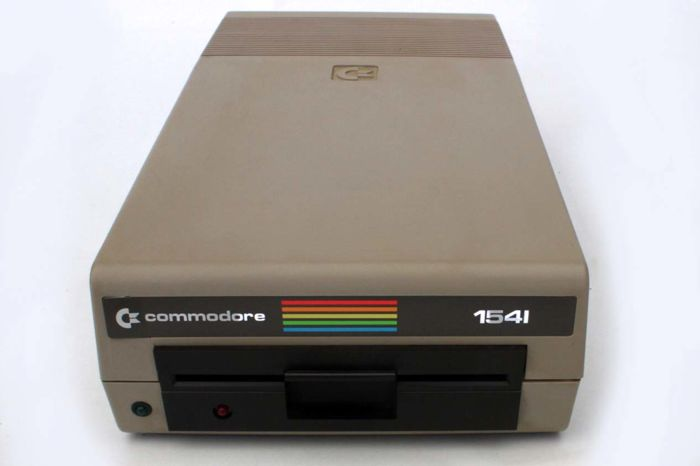
\includegraphics[width=\textwidth]{img/Commodore1541.jpg}
\caption[Commodore 1541 \textit{(preuzeto \cite{Commodore1541})}]{Commodore 1541}
\label{img:commodore1541}
\end{center}
\end{figure}

Originalna \textit{5.25" flopi disketa} ili \textit{miniflopi} bio je magnetni disk format koga je 1976. godine predstavio \textit{Shugart Associates} kao zamenu za 8-inčnu disketu koja se smatrala prevelikom za novije računare \cite{5.25Flopi}. Izgled diskete prikazan je na slici \ref{img:flopi}.

Osnovni oblik ove diskete imao je 35 kružnih traka dok je postojala i verzija sa 40 traka na kojima su bili raspoređeni sektori od po 256 bajta. Trake su imale različit broj sektora i bile su raspoređene od spolja ka unutra, odnosno prva traka je bila bliža spoljašnjoj ivici i imala je najviše sektora, dok je poslednja traka bila bliža unutrašnjem prstenu diskete sa najmanje sektora. Broj sektora po trakama je prikazan u tabeli \ref{tab:sektor_traka}.

\begin{figure}[ht]
\begin{center}
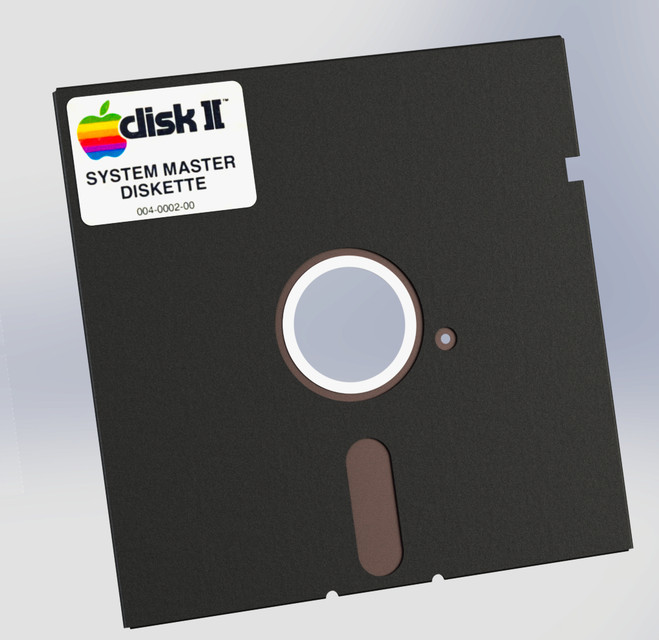
\includegraphics[width=13cm]{img/Flopi.jpg}
\caption[5.25" flopi disketa \textit{(preuzeto \cite{Flopi})}]{5.25" flopi disketa}
\label{img:flopi}
\end{center}
\end{figure}

\begin{table}[h!]
\begin{center}
\begin{tabular}{ | c | c| c | c | } 
\hline
Traka & Sektori/traka & Ukupno Sektora & Skladište u bajtima \\
\hline
\hline
1-17 & 21 & 357 & 7820 \\
\hline
18-24 & 19 & 133 & 7170 \\
\hline
25-30 & 18 & 108 & 6300 \\
\hline
31-35 & 17 & 85 & 6020 \\
\hline
\end{tabular}
\end{center}
\caption{Broj sektora po traci originalne \textit{5.25" flopi diskete}}
\label{tab:sektor_traka}
\end{table}

Traka 18 predstavlja glavnu traku sa svojih 19 sektora. Nulti sektor ove trake čuva BAM(Block Availability Map) i ime flopi diskete dok ostali sektori sadrže podatke. BAM je struktura podataka koja prati koji sektori traka su slobodni a koji zauzeti. Sektor u kome je smesten BAM je formiran po posebnom šablonu. BAM za prvu traku smešten je od 4-7 bajta nultog sektora. Gde prvi bajt govori ukupan broj slobodnih sektora, dok preostala tri govore koji sektori su slobodni a koji popunjeni. Svaka naredna 4 bajta predstavljaju BAM za narednu traku flopi diskete. 128 bajt čuva ime flopi diskete.

Podaci su uvek smešteni počevši od 1 sektora dok je nastavak na 4-tom ukoliko je reč o direktorijumima jer se pomeranje vrši za 3 sektora, dok se za smeštanje fajlova koristi pomeranje od 10 i u tom slučaju nastavak je na 10-tom sektoru. Sektori su popunjeni po šablonu, prva dva bajta sektora govore o lokaciji sledece trake/sektora. Kada dođemo do kraja direktorijuma vrednost prvog bajta je 00.

\textit{D64 fajl} je najšire podržani i dobro definisan format koji predstavlja elektronsku byte predstavu \textit{5.25"flopi diskete} za \textit{Commodore 64} računare. Standardni \textit{D64 file} ima 174848 bajtova, 683 sektora sa po 256 bajta i on oslikava originalnu \textit{5.25" flopi disketu} sa 35 traka.  Postoji i verzija ovog fajla sa 196608 bajtova,768 sektora sa po 256 bajta koja oslikava verziju \textit{5.25" flopi diskete} sa 40 traka.

Na kraju \textit{D64 fajla} mogu se naći dodatni bajtovi, koji govore koji sektori imaju grešku. Ukoliko se na kraju fajla ne pojave bajtovi to znači da su svi sektori ispravni. Svaki bajt je vezan za po jedan sektor odnosno koliko sektora flopi disketa ima toliko će imati i bajtova na kraju fajla ukoliko taj fajl ima gresku u nekom od sektora. U zavisnosti od broja traka i broj dodatnih bajtova se menja i to za 35 traka 689 bajtova dok je za 40 traka 768 bajtova. Ukoliko je vrednost bajta postavljena na 1 to znači da korespodentni sektor nema grešku \cite{D64}. Veličina fajlova u zavisnosti od dodatnih bajtova je prikazana u tabeli \ref{tab:error_velicina}.
\begin{table}[h!]
\begin{center}
\begin{tabular}{ | c | c |} 
\hline
Tip diskete & Veličina(bajt) \\
\hline
\hline
35 traka, no errors & 174848 \\
\hline
35 traka, 689 error bajtova & 175531 \\
\hline
40 traka, no errors & 196608 \\
\hline
40 traka, 768 error bajtova & 197376 \\
\hline
\end{tabular}
\end{center}
\caption{Veličina fajla u zavisnosti od dodatnih bajtova}
\label{tab:error_velicina}
\end{table}

\subsection{Problem}

% Istorija je pregazila ovaj medium
% Reci zbog cega se radi cuvanje u d64 formatima da se ne izgube podaci i sacuvaju od vremena
% Kao i da se obezbedi i zabelezi istorija ...

Prilikom čitanja \textit{5.25"flopi diskete} i njenog prebacivanja u elektronski oblik odnosno \textit{D64 fajl} dolazi do pojave grešaka na nekim sektorima. Nastale greške prilikom čitanja se skladište u dodatnaim bajtovima na kraju \textit{D64 fajla} i dalja evidencija grešaka se vrši isključivo preko ovih dodatnih bajtova.
\section{Opis korišćenih tehnologija i alata}

Programsko rešenje je razvijeno uz pomoć \textit{Java} programskog jezika i  \textit{Eclipse} programskog razvojnog okruženja prvenstveno namenjenog za razvoj \textit{Java} aplikacija. Pored \textit{Jave}, \textit{Eclipse} podržava i druge programske jezike \cite{Eclipse}. Izgled \textit{Eclipse} razvojnog okruženja je prikazan na slici \ref{img:eclipse}.

\begin{figure}[ht]
\begin{center}
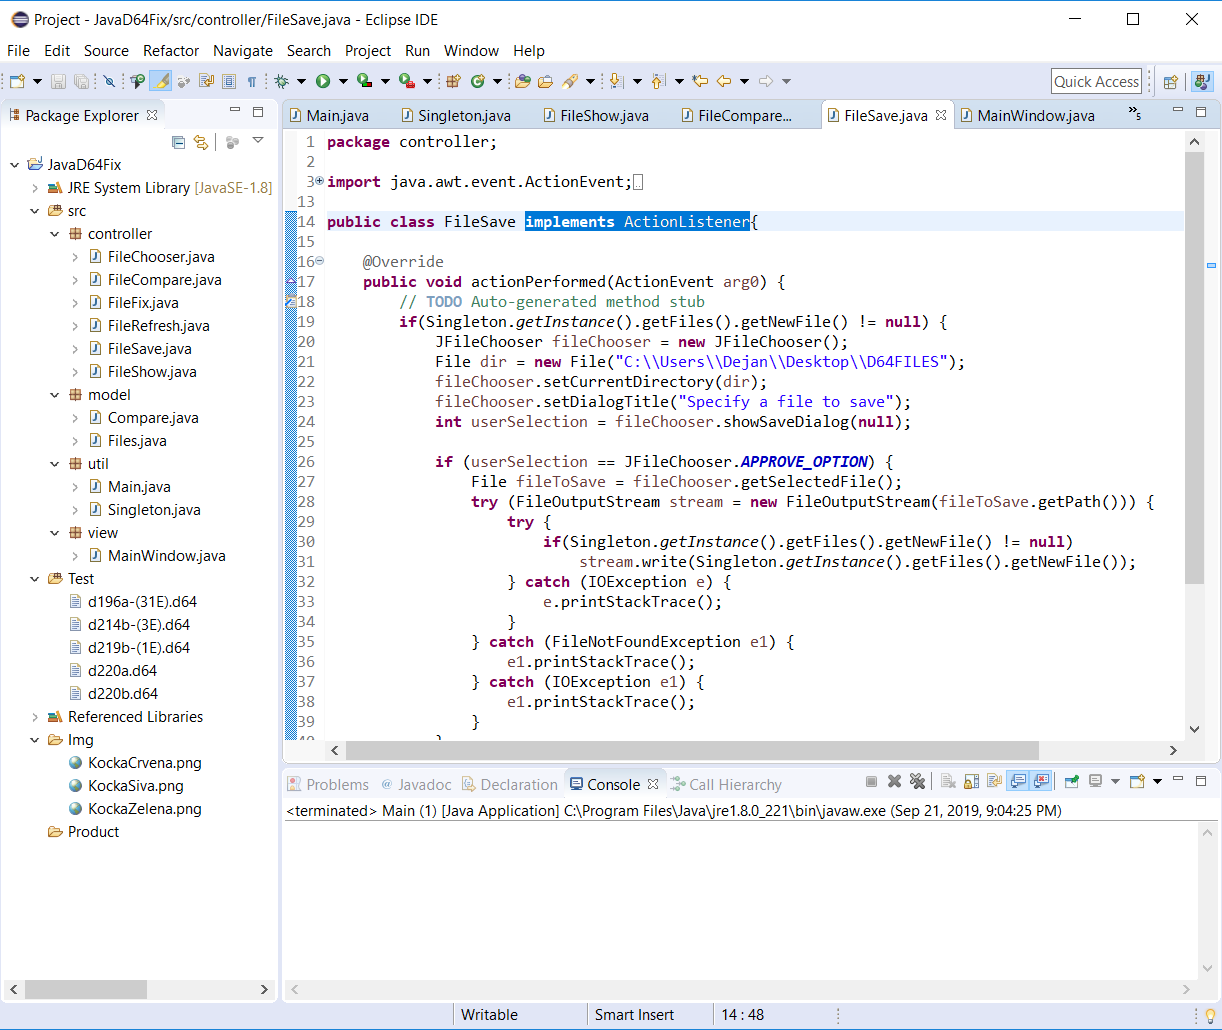
\includegraphics[width=\textwidth]{img/EclipseIDE.png}
\caption{Eclipse}
\label{img:eclipse}
\end{center}
\end{figure}

Za rad sa grafičkim elementima korišćen je \textit{Swing} radni okvir koji obezbeđuje skup grafičkih komponenti uz pomoć kojih realizujemo grafički korisnički interfejs u java programskom jeziku.
\section{Analiza citanja \textit{5.25" flopi disketa}}

\section{Rešenje problema}
\subsection{Opis rešenja problema}

Na osnovu analize \textit{D64 fajla} ustanovljeno je da se višestrukim čitanjem iste \textit{5.25 flopi diskete} dobijaju fajlovi sa greškama na različitim sektorima. Na osnovu ovoga konstruisano je rešenje gore opisanog problema koje je zasnovano na kombinaciji više \textit{D64 fajlova} sa ciljem da se kreira novi fajl koji bi imao manje ili u idealnom slučaju bio  bez grešaka. Suština postupka bi bila da se sektori koji imaju grešku zamene sa ispravnim sektoirma iz drugih \textit{D64 fajlova} iste \textit{5.25 flopi diskete} ukoliko oni postoje.

\subsection{Programsko rešenja problema}

Pošto svi fajlovi koji učestvuju u procesu imaju greške, algoritam počinje traženjem fajla koji ima najmanje grešaka jer to dalje smanjuje broj pretraga prilikom zamene sektora sa greškama. Dat je kod koji se bavi ovim procesom, gde se prvo učitavaju svi bajtovi tekućeg fajla i zatim u zavisnosti od dimenzija vrši se prebrojavanje sektora pod greškama i ukoliko taj fajl ima manje grešaka od trenutno najboljeg on se postavlja za novi najbolji. Postupak se ponavlja  po principu traženja minimuma odnosno fajla sa najmanje grešaka.

\begin{lstlisting}[language=Java]
byte[] newFile = null;
int best = 1000;
for (File file : Singleton.getInstance().getCompare()
                                    .getCompare()) {
    byte[] fileContent = null;
    try {
    	fileContent = Files.readAllBytes(file
    	                           .toPath());
    } catch (IOException e1) {
    	// TODO Auto-generated catch block
    	e1.printStackTrace();
    }
    
    if(fileContent.length == 175531) {
    	int temp = 0;
    	for(int i=fileContent.length-1 ; 
    	 i > fileContent.length-684 ; i--) {
            if(fileContent[i] != 1) {
            	temp++;
            }
        }
    	if(temp <= best) {
    		best = temp;
    		newFile = fileContent;
    	}
    }else if(fileContent.length == 197376){
    	int temp = 0;
    	for(int i=fileContent.length-1 ; 
    	i > fileContent.length-769 ; i--) {
            if(fileContent[i] == 1) {
            }else {
            	temp++;
            }
        }
    	if(temp <= best) {
    		best = temp;
    		newFile = fileContent;
    	}
    }else if(fileContent.length == 196608 
            || fileContent.length == 174848)
    	newFile = fileContent;
    	best = -1;
    }	
    Singleton.getInstance().getCompare()
                   .setFiles(fileContent);
}
\end{lstlisting}

Po pronalasku fajla sa najmanje grešaka, prolaskom kroz bajtove koji govore o greškama nad sektorima, uzimajući redom sektore sa greškama, proveravamo da li postoji fajl u kome je taj sektor ispravan. Ukoliko postoji vrši se kopiranje bajtova ispravnog sektora u bajtove neispravnog. Ovaj postupak se nastavlja do poslednjeg sektora sa greškama i u idealnom slučaju rezultuje fajlom bez grešaka.Dat je kod koji se bavi ovim postpukom za fajlove koji oslikavaju \textit{5.25 flopi disketu} sa 35 traka dok je za 40 traka postupak zansovan na istom principu samo sa različitim brojem dodatnih bajtova za greške.

\begin{lstlisting}[language=Java]
for(int i=newFile.length-683 
    ; i < newFile.length-1 ; i++) {
if(newFile[i] != 1) {
	for (byte[] b : Singleton
	.getInstance()
	.getCompare().getFiles()) {
		if(b[i] == 1) {
			for(int j = (i-174848)*256;
			j < (i-174848)*256+256 ; j++) {
				newFile[j] 
				    = b[j];
			}
			newFile[i] = 1;
			break;
		}
	}
}
}
\end{lstlisting}

\subsection{Prikaz implementiranog rešenja}

Početni izgled aplikacije prikazan je na slici \ref{img:aplikacija}. Klikom na dugme \textit{Select D64} vršimo izbor fajlova. Klikom na dugme \textit{Fix selected D64} pokreće se gore opisani algoritam za popravku selektovanih fajlova i interno kreiranje novog sa minimalnim brojem grešaka. Klikom na dugme \textit{Save D64} omogućava se čuvanje prethodno popravljenog i prikazanog fajla na lokaciji koju korisnik odabere. Klikom na dugme \textit{Refresh} vrši se deselekcija svih selektovanih fajlova kao i selekcija fajlova za prikaz.

Selekcija fajlova se vrši na osnovu čekera u levom donjem delu aplikacije a prikaz na osnovu radio dugmadi. Brojevi kod vizuelnog prikaza govore o kojoj traci \textit{5.25 flopi diskete} je reč dok donja traka služi za prikaz svih informacija bitnih za korisnika. Izgled ovog dela aplikacije prikazan je na slici \ref{img:aplikacija1}.

\begin{figure}[ht]
\begin{center}
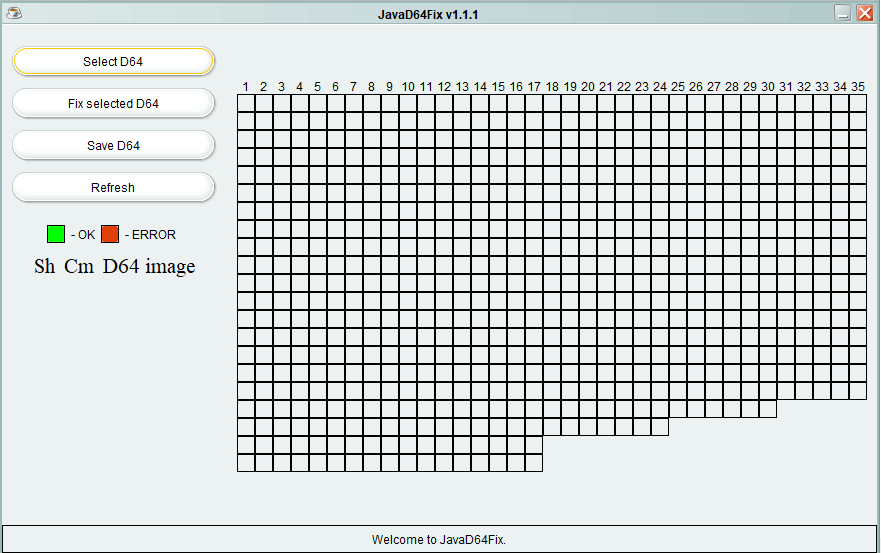
\includegraphics[width=\textwidth]{img/aplikacija.png}
\caption{Izgled aplikacije}
\label{img:aplikacija}
\end{center}
\end{figure}

\begin{figure}[ht]
\begin{center}
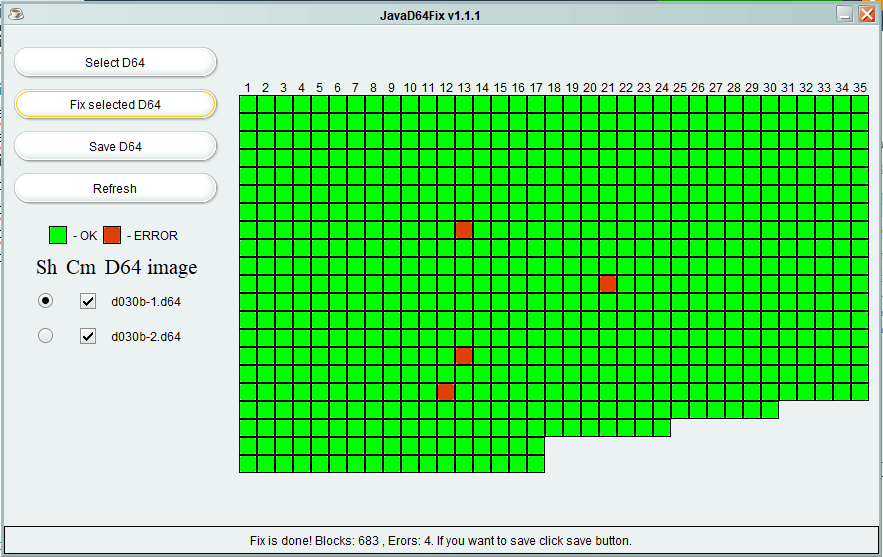
\includegraphics[width=\textwidth]{img/aplikacija1.png}
\caption{Izgled aplikacije}
\label{img:aplikacija1}
\end{center}
\end{figure}

\section{Zaključak}

U ovom radu predstavljeno je rešenje za problem lošeg čitanja \textit{5.25" flopi disketa} i njegovo pretvaranje u elektronski \textit{D64 fajl}. Opisan je kompletan postupak kojim je to postignuto kao i sve potrebne informacije za razumevanje problema i njegovo rešenje.

Rešenje je proizišlo iz detaljne analize D64 fajla kao i procesa čitanja podataka sa \textit{5.25" flopi diskete} gde je oučeno da se višestrukim čitanjem javljaju greške u različitim sektorima. Ova informacija bila je ključna prilikom otklanjanja ovog problema u većoj ili manjoj meri.

Proširenje datog programskog rešenja može se kretati u smeru vizualizacije izmenjenih sektora sa greškama u vidu prikaza podataka i ručnom kontrolom izmene istih, gde bi korisnik ovaj automatizovan proces mogao kontrolisati. Takođe prilikom nailaska na sektore koji ne mogu biti popravljeni korisnik bi dobio mogućnost da izabere i sa posmatranim sektorom zameni sektor sa najmanje oštećenja ili sa sektorom čiju grešku smatra najpovoljnijom iz njegovog aspekta gledanja.
\section{Literatura}

\renewcommand{\bibname}{}
\bibliographystyle{unsrt}
\bibliography{biblioteka}

\end{document}
